\documentclass[12pt]{report}
\usepackage[utf8]{inputenc} 
\usepackage[T1]{fontenc}
\usepackage{layout}
\usepackage{graphicx}
\usepackage{verbatim}
\usepackage{moreverb}

%page de garde 
\title{Technical Report of the First Phase of the Project}
\author{Pierre-Yves Hervo \\Polytech Nantes High school of Engineering }
\date{11th of July 2013}

\begin{document}
\maketitle

\begin{abstract}
This report explain how I managed to interface Praat and Java and how the Genetic Algorithm is implemented. The first part of this report will be an overAll to explain general concepts and the second part will deals with my particular Java implementation.

\paragraph*{}
Important: This solution is working on windows 7, it is supposed to work on Linux but it won't work on a Mac because of the Praat's API.

\end{abstract}

\tableofcontents

\part{Overall}

\chapter{About the Genetic Algorithm}
This chapter deals with the basics of how my genetic algorithm work. I will explain my implementation in the second part.

\section{Principle}
The Genetic Algorithm I use is based on the common genetic algorithm and I introduce some specificities in the fitness function. This section will present the common point with a classical GA and I will present the specificities in the next one.

\subsection{The target}
The best way to recognise a vowel is to compare the formants of the candidate sound to the formants of a well known sounds.

For example, if we want to know if a sound is a "i", we will compare the formants of the candidate sound to the values which are defined for a i.

We declared two formants for each sound. We choose two because some vowels only get two formants and if we look for three, Praat will produce an error. Each of this formant get a value for the frequency and a value for the bandwidth. Praat can easily calculate such data but we still haven't find a way to calculate the amplitude.

\subsection{The candidate}
We will compare the candidates formants to the reference formants. For that purpose, we need to synthesise the sound and calculate its formants. The software Praat will do both for us. The only thing we need to do is to send it a script with values for each parameter.

The problem of how to send this script will be solved in the next chapter.

\paragraph*{}
There is 29 parameters for voice synthesis in Praat. We use a linear voice synthesis which means that each parameters get two values to represent time evolution: one for the beginning 0.0 and one for the end, 0.5 in the figure below.

\begin{figure}[h]
\begin{center}
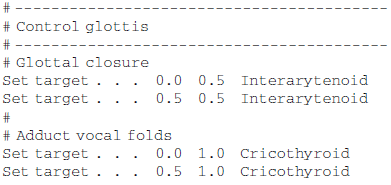
\includegraphics{resources/praatScript.png} 
\end{center}
\caption{Example of Praat script to set two variables. Source : \cite{ref5}}
\label{praatScript}
\end{figure}

So there is a lot of value to define. Fortunately, Praat will automaticly complete the values for some parameters by default, we will only need to define the 10 most important.

Which means that the structure we will make evolve int the GA is a structure containing 20 values, one for each parameter to set in the Praat script.

\subsection{Evolution Operators}
We use two common evolution operators for a GA : a one point cross over at each generation and then a mutation with a probability of 0.2 to append.


\section{Particularities}

\subsection{In the sequence generation}
The last point about the particularities is that we have a knowledge of how the speech synthesis work and we have an idea of the range of values for each parameter. It allow to use this knowledge to restrain the search domain without making the GA deterministic.
More details on the second part.

\subsection{In the fitness function}
The particularity of my Ga is located in the fitness function. I used another program (Praat) to execute a script. This script will generate a sound, analyse it to get the formants and then get the values back. Then I will compare the formant in the result from Praat with the formants given to the program as the target.

It is different from other fitness function that typically take care themselves of the calculation part. Here it delegate it to another program and only do a comparison.
It do it for each individual of the generation's population.

The formants values used as target are just a reference, they are not an exact value to reach. In practice, we can estimate that a formant value can increase or decrease over 10\% of this value. That's why the fitness function of my GA compare the values of the formants of the candidate and accept a value in the interval of +/-10\% of the values of the target's formants.

\section{Recap}
We have seen that the structure of my GA respect the general structure of a common GA with some particularities to adapt to the subject of speech synthesis.

As a recap, here is the algorithm :


\begin{verbatimtab}[3]
1) generate the candidate population with the reduced range values.
2) while not converge{
		a) For each individual of the population{
					-> generate Praat's script with values 
					-> make it executed by Praat
					-> get the formant values of generated sound back
					-> compare with the formants values of the target sound	   
		   }endFor
		   
		b)if no solution found then{ 
				cross over and mutation to get an evolved population.
			}else{
				 quite the while loop  	 
			}   
		
   }endWhile

\end{verbatimtab}

\chapter{How to connect Java and Praat}
Giving the Praat's API, we need to use two different ways to connect Java and Praat.
We need to consider one way to communicate between Java and Praat to send and execute the Praat script and another to send the response from Praat to Java.

\section{From Java to Praat}
We want to send a Praat's script to Praat and have it executed. The way I choose is the software SendPraat\cite{ref}. It is a program developed by the same authors as Praat. It allow to send orders to a {\bfseries running instance of Praat}\footnote{This is very important, if there is no Praat already launched, SendPraat won't work.}.
It means we need two programs :

\begin{enumerate}
\item a normal Praat software already launched.
\item SendPraat which will give it orders. No need to launch this one, it only works in command line.
\end{enumerate}

If you give SendPraat the name of a script, it will made Praat launch and execute it. The only thing left is to make Java executed SendPraat. For this, I used the Java Runtime Environment which can use the command line of windows. I will explain it in the second part of this report.

 and praat link in bibliography+ url

Note : I used a SendPraat.exe as I used windows but you can compile the source code yourself to use it in your own operating system. If you want to make Praat communicate with a C program, you can use the SendPraat directive, no need to compile source code. For more information, look at the Praat's API, section Praat scripting. As I was working in Java, the solution I presented is currently the best.

\section{From Praat to Java}
There is only one way to make Praat communicate with another program, whenever the language is, the sockets\footnote{It only work for windows and Linux, it is the Praat API wich manage it like this.}. 

Sockets are a way use in computer science to make two different program communicated. For this, they will use the network principles and send network packets to a computer on a specified port. It is not necessary that it was another computer, it can be the same and int that case, we use a local network call localhost. The first program will send a message to the other specifying the port and the second one will listen will listen to the port and get the message when it arrived.

Praat allows to send sockets by the directive "sendsocket" but it cant received sockets from another program. That is why we got to use the SendPraat program in the other side.
If Praat send a socket then our GA will need a functionality which always listen to this port and  will take the message. Such functionality basically call a {\bfseries Server}.
In that purpose, I implement a Java server that listen to a specific port. I will describe it in the second part of the report.

\section{Sequencing}
There is a problem of sequencing to take care to synchronise Java and praat. The problem came from the fact that it is two different thread(program) running.
They both have a different execution's speed. The Java's GA work very fast, each generation take a few seconds while each sound synthesis take a few seconds in Praat. For example, it take approximately 12 second to Praat to generate a 2.0 seconds sound.
So there is a problem of speed and synchronisation.

This is the reason why I should have establish a sequencing between the two programs to force the Ga to wait for Praat's answer before going to the next individual. More precisely to wait that the server get the answer from Praat and store it into the GA. The GA could do the comparison of formants while it is done.

The only solution was to use a semaphore. It is a computing technique for sequencing tasks. It work on the principle of token. You have a token in a box, if someone want to do an action he took the token and it released it when finished. The others wait for the token to be free before doing their action.
I used in fact two level of semaphore in the fitness function.
The first on is when the GA start the fitness function, it took the token and it released it when it had finished the comparison. If prevent the Ga to launch the fitness function with another candidate while still running the previous one. For example if Praat is still running a synthesis, it wont be able to do the comparison with a empty values and switch to the next candidate.

The second level is in the function fitness itself, it allow to be sure that the server had store the message into the GA. Has the server is a different thread, it is a obligation. It forbid the fitness function to do the comparison with the reference formant until a value was set by the server. It avoid errors.


\section{Recap}
So in conclusion we had to consider two different side for the communications : the message from Java to Praat and the message from praat to Java. On the first side, we had to use a specific praat program called SendPraat and on the other side we had to use a Java's Server to listen to Praat's sockets.

The figure below show how it works :
\begin{figure}
\begin{center}
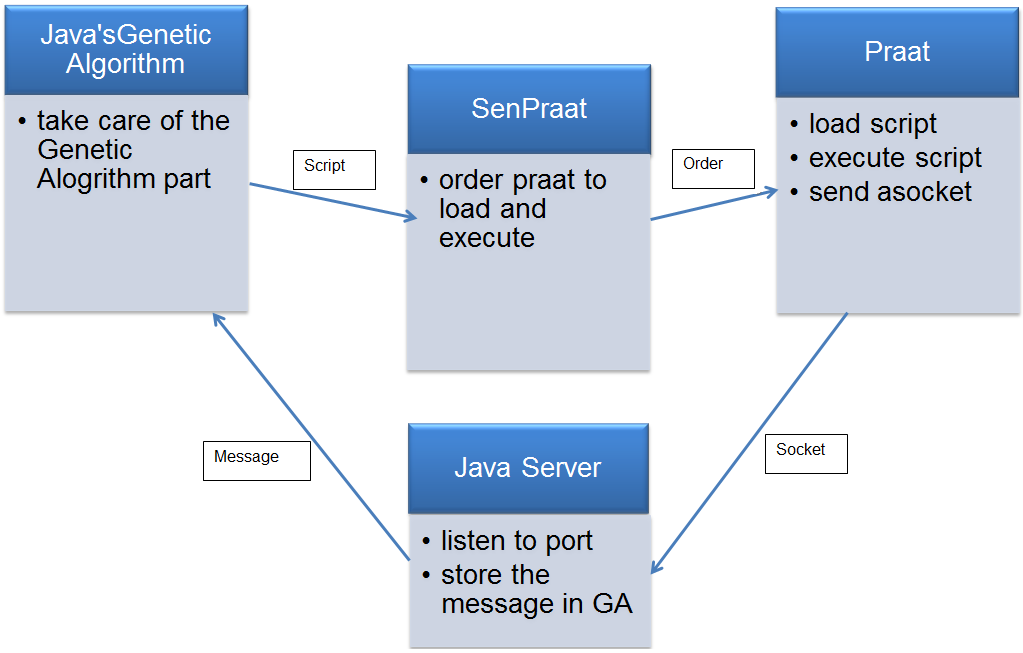
\includegraphics[scale=0.6]{resources/architecture.png} 
\end{center}
\caption{The exchange of information between Java and Praat and the role of each entity}
\label{architecture}
\end{figure}

\part{Implementation Details}
\chapter{the GA}
\section{watchmaker}
\section{basics elements to manipulate}
\section{the result}

\chapter{the communication}
\section{call to sendPraat}
\section{the server}
\appendix
\chapter{A scheme}

\listoffigures
\listoftables

\bibliographystyle{alpha} 
\bibliography{bib} % mon fichier de base de données s'appelle bibli.bib
\end{document}